%%%%%%%%%%%%%%%%%%%%%%%%%%%%%%%%%%%%%%%%%%%%%%%%%%%%%%%%
%   |------------------------------------------|       %
%   | Web App embebida en dispositivos móviles |       %
%   |  para la gestión de registros sobre la   |       %
%   |   contaminación de afluentes y ríos.     |       %
%   |                                          |       %
%   |          Proyecto de graduación          |       %
%   |__________________________________________|       %
%                                                      %
%   Autores                                            %
%   -------                                            %
%                                                      %
% * Bruno, Ricardo Hugo (CX 1409686)                   %
%     rburnount@gmail.com                              %
% * Gomez Veliz, Kevin Shionen (CX 1411828)            %
%     ing.gomezvelizkevin@gmail.com                    %
%                                                      %
%   Tutor                                              %
%   -------                                            %
%                                                      %
% * Ing. Cohen, Daniel Eduardo                         %
%        dcohen.tuc@gmail.com                          %
%                                                      %
%   Cotutor                                            %
%   -------                                            %
%                                                      %
% * Ing. Nieto, Luis Eduardo                           %
%        lnieto@herrera.unt.edu.ar                     %
%                                                      %
%                                                      %
%%%%%%%%%%%%%%%%%%%%%%%%%%%%%%%%%%%%%%%%%%%%%%%%%%%%%%%%

% ********* Introducción ********** %

%TODO: *Agregar Secciones de Android

\chapter{Introducción}
\label{chap:introduccion}

\begin{comment}
Requisitos del proyecto y los problemas a encarar
Razón de ser del proyecto: aplicación, investigación, etc.
Especificaciones generales del proyecto.


introducción es una sección inicial que establece el propósito y los objetivos de todo el contenido posterior del escrito. En general va seguido del cuerpo o desarrollo del tema, y de las conclusiones.

En la introducción normalmente se describe el alcance del documento, y se da una breve explicación o resumen de éste. También puede explicar algunos antecedentes que son importantes para el posterior desarrollo del tema central. Un lector al leer una introducción debería poder hacerse una idea sobre el contenido del texto, antes de comenzar su lectura propiamente dicha.

En artículos técnicos, la introducción generalmente incluye una o más sub-secciones estándar, como lo son el resumen o síntesis, el prefacio y los agradecimientos. Alternativamente, la sección de introducción puede ser un capítulo más del trabajo en sí, dividido en las sub-secciones anteriormente mencionadas. Cuando el libro se divide en capítulos numerados, por convención la introducción y cualquier otro asunto delante de las secciones de cuerpo o desarrollo no se enumeran (o se enumeran de manera distinta) y preceden al capítulo 1.

El concepto de introducción es independiente del contenido del documento al cual introduce. Siempre debe presentar el objeto o problema a desarrollar, ya este se trate de una especificación formal, un producto, un personaje o un ente cualquiera.
\end{comment}

La tecnología de los dispositivos móviles ha avanzado rápidamente en los últimos años, llegando a ser actualmente auténticas computadoras de bolsillo. La gran demanda por este tipo de dispositivos genera un gran interés por parte de empresas/instituciones que desean crear aplicaciones para un mercado en pleno auge, buscando aprovechar no sólo la gran cantidad de usuarios de estas plataformas, sino también la posibilidad de ofrecer funcionalidades y capacidades imposibles para sus procesos actuales.

% Muchas empresas comenzaron a desarrollar aplicaciones para teléfonos celulares y tablets como un complemento de sus sistemas existentes, haciendo que sea necesario que se desarrollen tecnologías para la comunicación entre la aplicación principal y los clientes que sean seguras y eficientes.

La plataforma que actualmente posee una mayor cantidad de usuarios y mayor crecimiento es Android, debido a que se trata de un Sistema Operativo abierto que cualquier fabricante puede adaptar e instalar en sus dispositivos, que está en constante evolución, y que aporta gran cantidad de servicios y aplicaciones. 

\section{Objetivos}

Los principales objetivos del sistema a desarrollar son permitir que usuarios puedan realizar el estudio de campo de una manera rápida y eficiente valiéndose de la tecnología de un smartphone, con cualquier SO instalado, que hoy en dia se realiza de forma manual con lápiz y papel.

El sistema cuenta de dos partes, una aplicación movil para generar registros de las muestras del estudio de campo, y una aplicación web para gestionar y administrar dichos registros.

El sistema debe ser seguro, escalable, de fácil mantenimiento y muy simple de usar. Se deben implementar mecanismos de seguridad que impidan la visualización o alteración indebida de los datos sensibles de cada usuario.

Nuestros objetivos personales son aplicar los conocimientos adquiridos a lo largo de la carrera, el aprendizaje del trabajo en equipo, la coordinación en el desarrollo y sumar experiencia y conocimientos.


\section{Android}
Android es un sistema operativo Open Source, para dispositivos móviles basado en Linux. La mayor parte de su código fue publicado por Google bajo la licencia Apache. Actualmente se lo puede encontrar instalado en teléfonos celulares, tablet PCs y televisores.

%La estructura del sistema operativo Android se compone de aplicaciones que se ejecutan en un framework Java de aplicaciones orientadas a objetos sobre el núcleo de las bibliotecas de Java en una máquina virtual Dalvik con compilación en tiempo de ejecución.

Las aplicaciones de Android normalmente están escritas en el lenguaje de programación orientado a objetos Java, aunque es posible utilizar frameworks para desarrollar aplicaciones en otros lenguajes, como HTML5+CSS3+Javascript o Python. Estas aplicaciones se ejecutan sobre una máquina virtual Dalvik, que está optimizada para requerir poca memoria y está diseñada para permitir ejecutar varias instancias de la máquina virtual simultáneamente, delegando en el sistema operativo subyacente el soporte de aislamiento de procesos, gestión de memoria e hilos.

Incluye una tienda de aplicaciones llamada Google Play Store, desarrollada por Google. Esta aplicación se encuentra instalada en la mayoría de los dispositivos Android y permite a los usuarios navegar y descargar aplicaciones publicadas por los desarrolladores.

Por otra parte, los usuarios pueden instalar aplicaciones desde otras tiendas virtuales (tales como Amazon AppStore o GetJar) o directamente en el dispositivo si se dispone del archivo APK de la aplicación.

% La compañía de investigación Canalys estimó en el segundo trimestre del año 2009 que Android tenía una cuota de mercado del 2,8\% de smartphones en todo el mundo. En el cuarto trimestre de 2010 esta cifra había aumentado al 33\% del mercado, convirtiéndose en la plataforma para smartphones más vendida. En el tercer trimestre de 2011 se estima que más de la mitad (52,5\%) del mercado de smartphones pertenece a Android. En el tercer trimestre de 2012 Android tenía una cuota del 75\% del mercado mundial de smartphones según la firma de investigación IDC. En la figura \ref{fig:ventas-android} puede verse la evolución de las ventas de teléfonos celulares según su sistema operativo.

% \begin{figure}[htbp]
%   \centering
%     %lo que agregué entre corchetes hace que el ancho de la imagen ocupe el 80% del área de texto. Si sacás eso la imagen no se redimensiona y se va de la hoja. Se puede usar algo parecido para limitar el alto si es necesario.
%     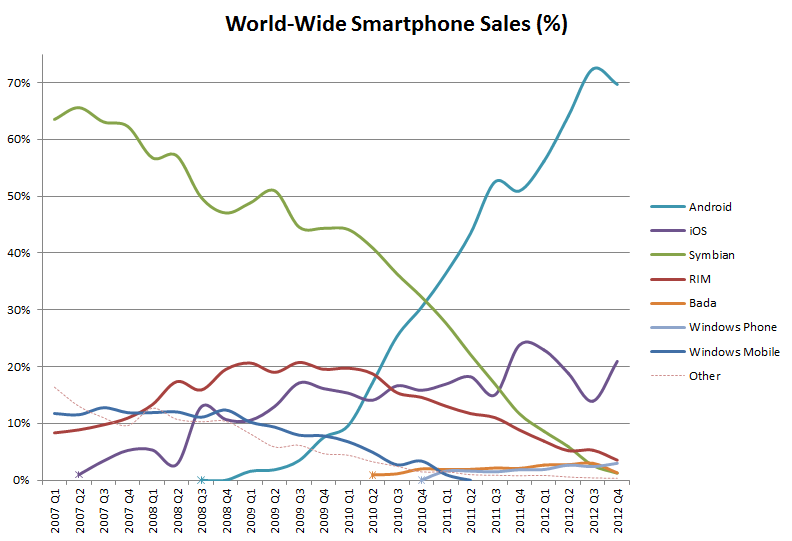
\includegraphics[width=0.8\textwidth]{imagenes/ventasAndroid.png}
%      \caption{Ventas de smartphones según su sistema operativo, a nivel mundial}
%     \label{fig:ventas-android}
% \end{figure}


% La cuota de Android en el mercado varía según la ubicación. En julio de 2012, la cuota de mercado de Android en los Estados Unidos fue de 52\%, y se eleva al 90\% en China.

\section{Desarrollo de Software}

Para resolver un problema, se sigue un Proceso de Resolución:

\begin{enumerate}
    \item Identificar el problema.
    \item Definir y Representar el problema.
    \item Explorar las posibles estrategias.
    \item Aplicar y mejorar las estrategias.
    \item Mirar atrás y Evaluar los efectos de la actividad realizada.
\end{enumerate}

El proceso de resolución de problemas software abarca:

\begin{enumerate}
    \item Análisis y especificación de requisitos (qué)
    \item Diseño del sistema Software (cómo)
    \item Codificación (realización del cómo)
    \item Pruebas
    \item Instalación (la solución debe ser usada)
\end{enumerate}

\section{Análisis y Diseño Orientado a Objetos}

El análisis se enfoca en la investigación de los problemas y los requisitos, más que en la solución. Es un término utilizado, por ejemplo, en el análisis de requisitos (una investigación de los requisitos) o análisis orientado a objetos (una investigación de los objetos de dominio).

Durante el análisis orientado a objetos, se trata de encontrar y describir los objetos o conceptos en el dominio del problema.

El diseño tiende a una solución conceptual (de software y hardware) que cumpla los requisitos, en lugar de su implementación. Los diseños pueden ser implementados, y la implementación (como ser el código) expresa el diseño realizado, verdadero y completo.
El término es muy utilizado, como en el diseño orientado a objetos o el diseño de bases de datos.

Durante el diseño orientado a objetos, se procura definir objetos de software, y cómo ellos colaboran para satisfacer los requisitos.

\section{Lenguaje de Modelado Unificado (UML)}

UML es un lenguaje estándar de diagramación. Puede ser usado para visualizar, especificar, construir y documentar los artefactos de un sistema de software.

Hay tres maneras de aplicar UML:

\begin{itemize}
    \item \emph{Como boceto:} Diagramas  informales e incompletos (frecuentemente dibujados en pizarras blancas) creados para explorar partes dificultosas del espacio del problema o de la solución, aprovechando el poder de los lenguajes visuales.
    \item \emph{Como plano:} Diagramas de diseño relativamente detallados, usados para:
        \begin{itemize}
            \item Ingeniería inversa para visualizar y entender mejor el código existente en diagramas UML.
            \item Generación de código. (ingeniería hacia adelante). Antes de programar, algunos diagramas detallados pueden proveer una guía para la generación de código (ej. Java), manualmente o automáticamente con una herramienta. 
        \end{itemize}
    \item \emph{Como lenguaje de programación:} Especificación ejecutable completa, de un sistema software en UML. El código ejecutable es automáticamente generado.
\end{itemize}

\textbf{En el presente proyecto, en general se procuró usar UML para la diagramación de bocetos, con un enfoque ágil, para la comunicación entre los miembros del equipo, y la resolución de distintos problemas, a lo largo de las disciplinas del proceso.
Sin embargo, algunos diagramas se realizaron con bastante detalle, utilizando herramientas CASE de UML  para la documentación de casos relevantes y para la posterior generación de código.}

Una misma notación puede ser usada para tres perspectivas y tipos de modelos:

\begin{itemize}
    \item \emph{Perspectiva conceptual:} Los diagramas son interpretados como cosas descriptas en una situación del mundo real o dominio de interés.
    \item \emph{Perspectiva de especificación (software):} Los diagramas describen abstracciones o componentes de software con especificaciones e interfaces, pero no obligadas a una implementación particular.
    \item \emph{Perspectiva de implementación (software)} Los diagramas describen implementaciones de software en una tecnología particular.
\end{itemize}

\textbf{Las tres perspectivas se aplicaron a lo largo del proceso de desarrollo del sistema.}

\section{Algunas definiciones}
\begin{itemize}
    \item \emph{Análisis Orientado a Objetos (AOO):} El AOO es un método de análisis que examina los requisitos desde la perspectiva de las clases y objetos que se encuentran en el vocabulario del dominio del problema.
 
    \item \emph{Diseño Orientado a Objetos (DOO):} El DOO es un método de diseño que abarca el proceso de descomposición orientada a objetos y una notación para describir los modelos lógico y físico, así como los modelos estático y dinámico del sistema que se diseña.

    \item \emph{Programación Orientada a Objetos (POO):} La POO es un método de implementación en el que los programas se organizan como colecciones cooperativas de objetos, cada uno de los cuales representa una instancia de alguna clase, y cuyas clases son, todas ellas, miembros de una jerarquía de clases unidas mediante relaciones de herencia.

    \item \emph{Proceso Software:} colección de actividades que comienza con la identificación de una necesidad y concluye con el retiro del software que satisface dicha necesidad.

    \item \emph{Ciclo de vida:} la transformación que el producto software sufre a lo largo de su vida, desde que nace (o se detecta una necesidad) hasta que muere (o se retira el sistema).

    \item \emph{Estados:} resultado de las transformaciones que sufre el producto software a lo largo de su ciclo de vida y representan en esencia el producto mismo.

    \item \emph{Modelo de ciclo de vida:} es la representación descriptiva y prescriptiva del ciclo de vida que indica el orden cronológico en el que deben llevar a cabo las actividades del proceso software. Un ciclo de vida debe determinar el orden de las fases del proceso software y establecer los criterios de transición para pasar de una fase a la siguiente.
 
    \item \emph{Disciplina:} Una colección de actividades relacionadas con un área de interés importante dentro del proyecto global.
    
\end{itemize}

\section{Ciclo de vida Iterativo Evolutivo}

\begin{quote}
“Deberías usar un desarrollo iterativo sólo en los proyectos que quieras que tengan éxito” - Martin Fowler
\end{quote}

El desarrollo iterativo evolutivo, en contraste con el ciclo de vida de cascada o secuencial, consiste en la programación y pruebas tempranas de un sistema parcial, en ciclos repetitivos. También normalmente supone que el desarrollo se inicia antes de que todos los requisitos se definan en detalle; el feedback se utiliza para aclarar y mejorar las características cambiantes.

Cuenta con pasos de desarrollo cortos y rápidos, feedback, y adaptación para aclarar los requisitos y el diseño, sin tanta especulación antes de la programación, como en método de cascada. La investigación demuestra que los métodos iterativos se asocian con mayores tasas de éxito y de productividad, y bajos niveles de defectos.

En este ciclo de vida, el desarrollo está organizado en una serie de mini-proyectos cortos y de longitud fija (timeboxing), llamados iteraciones; el resultado de cada uno es un sistema parcial probado, testeado e integrado. Cada iteración tiene sus propias actividades de análisis de requisitos, diseño, implementación y pruebas.

El ciclo de vida iterativo se basa en la ampliación y refinamiento sucesivos de un sistema a través de múltiples iteraciones, con retroalimentación cíclica y adaptación, como conductores principales para converger al sistema  adecuado. Como el sistema crece gradualmente con el tiempo, iteración por iteración, se lo llama desarrollo iterativo e incremental. Y debido a que la retroalimentación y la adaptación producen una evolución en las especificaciones y el diseño, también es conocido como desarrollo iterativo y evolutivo.

La salida de una iteración no es un prototipo experimental o desechable, y el desarrollo iterativo no es prototipado. Por el contrario, la salida es un subconjunto, en calidad de producción, del sistema final.

\subsection{Beneficios}
\begin{itemize}
    \item Menos fracasos de proyectos, mejor productividad y tasas de defectos reducidas; demostrado por investigación de métodos iterativos evolutivos.
    \item Mitigación temprana, más que tardía, de altos riesgos (técnicos, requisitos, objetivos, usabilidad, etc.)
    \item Progreso visible y temprano.
    \item Feedback, compromiso de usuario, y adaptación tempranos, llevando a un sistema refinado que satisface más estrechamente las necesidades reales de los clientes.
\end{itemize}

Según nuestra propia experiencia, una ventaja adicional es que nos permitió refinar además nuestras propias actividades, mejorando la productividad, estimación, diagramación y calidad del desarrollo en cada iteración.

\textbf{Siguiendo recomendaciones de metodologías ágiles, trabajamos con ciclo de vida iterativo evolutivo.}

\section{Proceso Unificado (UP)}

Un proceso de desarrollo de software describe un enfoque para la construcción, despliegue, y posiblemente mantenimiento del software.

El Proceso Unificado nació como un popular proceso de desarrollo iterativo para la construcción de sistemas orientados a objetos. Es un marco de desarrollo de software que se caracteriza por estar dirigido por casos de uso, centrado en la arquitectura y por ser iterativo e incremental.\\[5cm]

\begin{figure}[htbp]
  \centering
    %lo que agregué entre corchetes hace que el ancho de la imagen ocupe el 80% del área de texto. Si sacás eso la imagen no se redimensiona y se va de la hoja. Se puede usar algo parecido para limitar el alto si es necesario.
    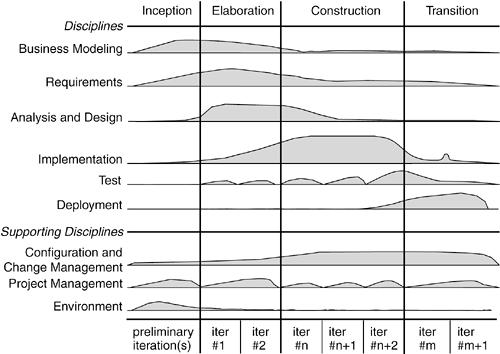
\includegraphics[width=0.8\textwidth]{imagenes/rup}
        \hfill
	\caption{Disciplinas y fases del Proceso Unificado}
	\label{fig:rup}
\end{figure}

\subsection{Características}
    
\begin{itemize}
    \item \emph{Iterativo e Incremental:} Es un marco de desarrollo iterativo e incremental compuesto de cuatro fases denominadas Inicio, Elaboración, Construcción y Transición. Cada una de estas fases es a su vez dividida en una serie de iteraciones. Estas iteraciones ofrecen como resultado un incremento del producto desarrollado que añade o mejora las funcionalidades del sistema en desarrollo. Cada una de estas iteraciones se divide a su vez en una serie de disciplinas. Aunque todas las iteraciones suelen incluir trabajo en casi todas las disciplinas, el grado de esfuerzo dentro de cada una de ellas varía a lo largo del proyecto.
    \item \emph{Dirigido por los casos de uso:} Los casos de uso se utilizan para capturar los requisitos funcionales y para definir los contenidos de las iteraciones. La idea es que cada iteración tome un conjunto de casos de uso o escenarios y desarrolle todo el camino a través de las distintas disciplinas: diseño, implementación, prueba, etc.
    \item \emph{Centrado en la arquitectura:} Asume que no existe un modelo único que cubra todos los aspectos del sistema. Por dicho motivo existen múltiples modelos y vistas que definen la arquitectura de software de un sistema.
    \item \emph{Enfocado en los riesgos:} Requiere que el equipo del proyecto se centre en identificar los riesgos críticos en una etapa temprana del ciclo de vida. Los resultados de cada iteración, en especial los de la fase de Elaboración, deben ser seleccionados en un orden que asegure que los riesgos principales son considerados primero.
    \item \emph{UML:} Hace uso extensivo de diagramas UML para sus artefactos.
\end{itemize}

\textbf{Se trabajó sumando al proyecto, para cada iteración, un porcentaje (30\% aprox.) del total de casos de uso previstos.  A medida que se iba iterando se desarrollaban las disciplinas para estos nuevos casos de uso y se refinaban los casos de uso agregados en iteraciones anteriores, gracias a la experiencia adquirida y con la ayuda del feedback del usuario final.}



